\documentclass[acmtocl]{acmtrans2m}
%&t&{\tt #}&
%&v&\verb|#|&

% fancybox prevents the TOC from printing
%\usepackage{fancyhdr, fancybox, tabularx, verbatim, epsfig}
\usepackage{fancyhdr, tabularx, verbatim, epsfig}
\usepackage{amssymb,psboxit}
\usepackage{rotating}
\usepackage{tabularx}

\acmVolume{0}
\acmNumber{0}
\acmYear{00}
\acmMonth{00}

\newtheorem{interface}{Interface}[section]
\newtheorem{remark}{Remark}

\newcommand{\BibTeX}{{\rm B\kern-.05em{\sc i\kern-.025em b}\kern-.08em
    T\kern-.1667em\lower.7ex\hbox{E}\kern-.125emX}}

\markboth{M. Sala and K. Stanley}{Interfaces to Sparse Direct Solvers}

\title{On the Design of Interfaces to Sparse Direct Solvers}

\author{Marzio Sala and Ken Stanley}

\begin{abstract}
We report on the design of general, flexible, consistent, reusable and efficient
interfaces to direct solution software libraries for 
systems of linear equations on both serial and distributed memory
architectures. We present a set of abstract classes to access
the linear system matrix elements and its distribution, access to vector
elements, and control the solution of the linear system.

We describe a concrete implementation of the proposed interfaces, and we
report numerical results that show that the overhead induced by the
object-oriented design is negligible
under certain conditions. We report examples of applications using the
presented interfaces, and we comment
on the advantages and limitation of the design.
\end{abstract}

\category{D.1.3}{Programming Techniques}{Parallel Programming}
\category{D.2.2}{Software Engineering}{Design Tools and Techniques--{\sl
 Object-oriented design methods}}
\category{D.2.13}{Software Engineering}{Reusable Software--{\sl Reusable
  libraries}}
\category{G.1.3}{Numerical Analysis}{Numerical Linear Algebra--{\sl 
  Sparse, structured, and very large systems (direct and iterative methods)}}
%\terms{Documentation, Languages}

\keywords{Direct Solver Libraries, Object-Oriented Design, Distributed Linear Algebra.}
\begin{document}


\setcounter{page}{1}

\begin{bottomstuff}
Author's address:   \\
Marzio Sala: ETHZ/COLAB, Universit\"atstrasse 6, 8092, ETH Zentrum, Z\"urich,
  Switzerland. \\
Ken Stanley: FIXME
\end{bottomstuff}

\maketitle

% --------------------------------------------------------------------------- %
\section{Motivations}
\label{sec:introduction}
% --------------------------------------------------------------------------- %

This paper describes the design and the implementation of 
interfaces to serial and parallel direct solution libraries for
sparse linear systems of type
\begin{equation}
  \label{eq:linear_system}
  A X = B,
\end{equation}
where $A \in \mathbb{R}^{n \times n}$ is a real, square matrix, 
  and $X, B \in \mathbb{R}^{n}$ are the solution and
right-hand side vectors, respectively. 

Generally speaking,
a direct solution algorithm for (\ref{eq:linear_system}) is any 
technique that defines three matrices, $L$, $D$ and $U$, so that
$A = L \, D \, U$, and the linear systems with matrices $L$, $D$ and $U$ are
easy to solve. Generally, $L$ is a lower triangular matrix, $U$ is an
upper triangular matrix, and $D$ is a diagonal matrix 
(or possibly the identity matrix), and the algorithm adopted for their
computation is some variant of the Gaussian elimination. 
The development and implementation of
direct solvers for (\ref{eq:linear_system}) is a
challenging task that has been a subject of research for the
past four decades. 
We report in
Section~\ref{sec:overview} a brief overview of direct solution algorithms and
the corresponding software libraries.

\smallskip

Direct solution methods are required by several numerical algorithms, even
within the same application. An
incomplete list would include implicit time-marching schemes, 
Newton-like methods, multilevel and domain decomposition preconditioners. In
this article we focus on the {\sl usage} of direct solver libraries, and not
on their development or analysis. The point of view is the one
of application developers, interested in solving
(\ref{eq:linear_system}) using state-of-the-art software libraries.  

Unfortunately, for (distributed) sparse linear systems there is no direct
solve library of choice. This is in contrast with serial dense solvers, where
one can take advantage of the widely-available suite of solvers of the LAPACK 
library~\cite{lapack-guide}, of with distributed dense solvers, where one can
adopt the ScaLAPACK library~\cite{scalapack-guide}.

Since no ``gold standard'' exists, application developers aiming to solve
(\ref{eq:linear_system}) have to select one the several available libraries,
  then write a custom-made interface between the selected library and
  their application. This usually requires to store the linear system matrix using the
  storage format required by the library, then call the correct sequence of
  instructions to factorize the matrix and solve the linear system.  In our
  opinion, the approach is non-optimal for both application and library
  developers because it:
\begin{itemize}

\item 
{\sl offers partial coverage}. Writing a custom-made interface means that only the
targeted library will be used, while all others will be discarded.
This is inconvenient because 
it is often difficult to choose {\sl a-priori} the best library for a given
application.
In some cases, a theoretical analysis of
the problem at hand can suggest the right algorithm; alternatively, one can
consider numerical comparison available in the literature
on test matrices. Often, however, one has to validate
a given library on the application, architecture, and data
set of interest, and this can be done only if an interface  to a library
implementing the given method is already available;

\item 
{\sl produces maintenance problems.}
Including the interfaces within the application code requires the application
developers to take care of several details, like matrix format, memory
management, calling sequence, header files, and so on, that can vary 
from one version to the following. Although not necessary difficult, these
activities are usually time-consuming, and shift the focus of the application
developers;

\item 
{\sl slows down the usage of new libraries.} Since any new library 
(or a new version of a given library) may require a new matrix format or
distribution, or a new calling sequence, users may simply decide to continue
using the interface already developed.
\end{itemize}

This article shows that it is possible to overcome all these problems by using
modern software techniques, in the form of object-oriented (OO) design and
programming.  We propose a set of clean, consistent and easy-to-use interfaces
between the application and the direct solver libraries.  Each interface takes
care of dealing with the direct solver library, in a manner that is
transparent to the application developer, and automatically manage matrix
formats, data layout, calling sequences, and all the other ``details''
required by the supported libraries. 

\smallskip

We will present our design as a set of C++ classes. We adopted C++ because it
supports object-oriented design, and it is relatively easy to interface
FORTRAN77, FORTRAN90 and C libraries with C++ code. C++ is nowadays a common
choice for developers  of scientific libraries and applications, and several
projects have adopted C++ as the language of
reference~\cite{heroux05trilinos}. 
As regards the model of parallel computing,
we consider parallel architectures with distributed memory, and we suppose
that a message passing interface (usually MPI~\cite{gropp98mpi}) is adopted.
This approach is followed by the most important scientific libraries currently
available~\cite{heroux05trilinos,petsc-user-ref,falgout02hypre}; as a result, the presented
design can be easily interfaced with the aforementioned projects.

\smallskip

The paper is organized as follows. Section~\ref{sec:overview} introduces the
basic concepts of direct solution algorithms. Section~\ref{sec:design}
describes the requirements and the design of the proposed
interfaces. A concrete implementation is addressed in
Section~\ref{sec:concrete}. Section~\ref{sec:numerical} reports some
numerical results that quantify the overhead required by the generality of
the approach. Two
examples of application are reported in Section~\ref{sec:example}.
Section~\ref{sec:conclusions} outlines the conclusions.

%-----------------------------------------------------------------------------
\section{Overview of Direct Solution Methods}
\label{sec:overview}
%-----------------------------------------------------------------------------

{\bf Ken, this section still needs fixes, citations, and perhaps it should
  be condensed to shorten the article... I added at the end a table of some
    solvers, basically copied from Tim Davis' table -- maybe we should modify
the table and delete some of the information that are not useful to us...
Equation (\ref{eq:orig_eq}) should maybe be a reference to
(\ref{eq:linear_system}) to avoid repetitions...}

Direct solvers use Gaussian elimination (\ref{eq:ldu}) followed by a
forward solve (\ref{eq:forward}) and a backsolve (\ref{eq:backward})
to solve a system of linear equations (\ref{eq:orig_eq}):

\begin{eqnarray}
  \label{eq:orig_eq}
  A X = B \\ 
  \label{eq:ldu}
  PAQ = LDU \\
  \label{eq:forward}
  LX_1 = PB \\
  \label{eq:backward}
  UQ^{-1}X = D^{-1}X_1  
\end{eqnarray}

Where: $P$ and $Q$ are permutations.  $L$ and $U$ are lower and upper triangular, respectively.  And, $D$ is diagonal (often the identity matrix).  

If $A$ is sparse, $L$ and $U$
are typically sparse, though they may have some fill-in, i.e. non-zero entries which are zero in
$PAQ$.  

In a typical solver for an unsymmetric matrix, the column permuation,
$Q$ is chosen to minimze fill-in, while $P$, the row permutation, is
chosen to maintain numerical stability.  

Most direct solvers perform Gaussian elimination ($LU$ decompostion) in
two phases.  Symbolic factorization analyzes the matrix (typically
looking only at the structure or non-zero pattern of the matrix).
Numeric factorization uses the information from the symbolic
factorization phase, usually including a fill reducing column permutation, 
to improve performance.  

The performance of a sparse direct solver depends on the underlying
matrix, computer, application, algorithms, and libraries as well as
the code and how it is compiled.  Although a solver designed for an
unsymmetric matrix will work on symmetric matrices, solvers designed
for symmetric matrices will typically be faster on symmetric matrices.
Codes designed for shared memory computers will not run on distributed
memory computers.  Codes designed for distributed memory computers can
work on shared memory computers, but cannot take full advantage of the
shared memory architecture.  Many applications require repeated solves
with little or no difference in the matrix between solves.  Some
algortihms are able to take advantage of the similarity in matrices
between solves.

The different charasteristics of the matrices which users wish to
solve impact sparse direct solvers.  Some matrices are symmetric in both
structure and data $A_{i,j} = A_{j,i}$ for all $i$ and $j$.  Some of
the symmetric matrices are positive definite, SPD, and require no
pivoting.  The most efficient algorithms for symmetric and SPD
matrices will not work on other matrices.  Some are symmetric in
structure, $A_{i,j} == 0$ iff $A_{j,i} == 0$, or nearly so.
Algorithms that maintain symmetry typically outperform others on
matrices with symmetric or nearly symmetric structure.  Some have many
columns and/or rows that are structurally identical, or nearly so.
Aggregating nearly identical rows and columns into blocks allows more
efficient BLAS3 routines to be used.  Some can be factored with little
fill-in, others require significant fill-in.  Matrices that can be
factored with litte fill-in and have few identical or nearly identical
rows and columns are best handled by a low overhead code that does not
use the BLAS.  Some matrices are banded or nearly so, allowing the use
of a banded solver.  Matrices that have a non-trivial reduction to
block triangular form can be solved more quickly, often dramatically,
by a solver that includes reduction to block triangular form.  No sparse direct solver is best for all types of matrices.  

Some sparse direct solvers are designed for single processor
computers, some are designed for shared memory computers and others
are designed for distributed memory computers.  Solvers designed for
single processor computers can, if they use the BLAS for much of their
computation will achieve some speedup on shared memory computers.
Likewise, solvers designed for distributed memory computers can work
on shared memory computers using an MPI interface.  However, only
codes designed for shared memory computers can take advantage of the
shared memory architecture.  But, codes designed for shared memory
computers will not work on distributed memory computers.  No single
code will provide optimal performance across all architectures.

Some solvers handle certain application requirements better than
others.  Most aplications perform a series of solves, possibly
involving similar or even identical matrices.  If the matrix does not
change between two consequetive solves, the symbolic and numeric
factorization phases need not be performed for each solve.  If the
structure of the matrix does not change between consequetive solves,
but the values do, the numeric factorization must be performed for
each solve, though the symbolic factorization phase need not be.  If
the matrix values change, but the change is modest, the pivot order
may not need to change.  Therefore, some applications care most about
the execution time of the solve phase, while others are most sensitive
to the execution time of the factorization (numeric and/or symbolic).
Some applications require more accuracy than others.

\bigskip

Sparse direct solvers are complex codes which use a number of
strategies to reduce memory and time costs.  Pivoting for numerical
stability makes it impossible to know in advance how the algorithm
will proceed and requires a flexible data structure.  This is
particularly difficult for distributed memory codes.  

Solvers use different strategies to reduce fill-in.  Many ordering
methods exist to reduce fill-in and most sparse direct solvers support
more than one.  Some solvers will even choose an ordering method for
you.  There are multiple variations on minimum degree orderings: AMD,
COLAMD, MMD and variants within these.  Graph partitioning algorithms
result in bi-section or multi-section based orderings.  Solvers
designed for symmetric and nearly symmetric matrices typically use
symmetric permutations to maintain symmetry.  No single ordering
method s best for all matrices, nor has a heuristic been found that
consistently chooses the best ordering.

Since pivoting adds complexity which significantly increase execution
time, many solvers offer options to reduce the cost of pivoting.  Some
equilibrate the rows and columns of the matrix to improve diagonal
dominance.  Many codes will consider the effect on execution time when
choosing a pivot, accepting some loss of numerical stability.
Typically this just means accepting the diagonal pivot if it is within
some threshold of the best available, but some codes will take the
predicted effect on execution into consideration when choosing an off
diagonal pivot.

Some codes combine similar rows and columns into blocks to improve
locality and allow high performing BLAS to be called.  Some combine
only rows and columns that are identical, others will accept minor
differences in the rows and columns that they treat as blocks.  Such
blocking can reduce the cost of symbolic factorization as well.

The three common methods for exploiting parallelism are the
multi-frontal method, coalescing  similar 
columns into blocks and calling a parallel dense solver 
to factor the final block of the matrix.

Some solvers allow incomplete factorizations which ignore small
elements in the original matrix and/or the $L$ and $U$ factors.
This feature is used primarily by users seeking a
preconditioner for an iterative method.

Some solvers use iterative refinement to improve accuracy.  Iterative
refinement is used most often with codes that do not perform full partial pivoting.  

Given the differences in matrix, computer, application, algorithms,
and libraries, it is unlikely that a single sparse direct solver will 
outperform all others across all usages.  

Table~\ref{tab:packages} reports some of publicly available packages for
direct solution of linear systems.
For comparison, we refer for instance to
  \cite{amestoy01analysis,gupta01recent} and the references
  therein for more details and comparisons on the algorithms.

\begin{sidewaystable}[tbhp]
\begin{center}
\begin{tabular}{| l | c c c c | c c c c l l | p{5cm} |}
\hline
package & 
\rotatebox{90}{LU} &
\rotatebox{90}{Cholesky} &
\rotatebox{90}{$L D L^T$} &
\rotatebox{90}{QR} &
\rotatebox{90}{complex} &
\rotatebox{90}{BLAS} &
\rotatebox{90}{parallel} &
\rotatebox{90}{out-of-core} &
\rotatebox{90}{language} &
method &
references \\
\hline
%
CHOLMOD     & --        & $\bullet$ & -- & --        & $\bullet$ & 3  & -- & -- & C & left-looking supernodal & \cite{cholmod} \\
%
DCSPACK     & --        & $\bullet$ & 1  & --        & $\bullet$ & 3  & -- & D & C & multifrontal & \cite{dscpack-manual} \\
%
KLU         & $\bullet$ & --        & -- & --        & $\bullet$ & -- & -- & -- & C & left-looking & \cite{klu} \\
%
Mathematica & $\bullet$ & $\bullet$ & -- & --        & $\bullet$ & 3 & -- & -- & -- & various & \cite{mathematica} \\
%
MATLAB      & $\bullet$ & $\bullet$ & -- & $\bullet$ & $\bullet$ & 3 & -- & -- & -- & various & \cite{matlab} \\
%
MUMPS       & $\bullet$ & $\bullet$ & 1  & --        & $\bullet$ & 3 & D & -- & F90 & multifrontal & \cite{mumps} \\
%
Oblio       & --        & $\bullet$ & 2 & --         & $\bullet$ & 3 & -- &
$\bullet$ & ?? & left, right, multifrontal & \cite{oblio} \\
%  
PARDISO     & $\bullet$ & $\bullet$ & 2  & --        & $\bullet$ & 3 & S & --
& C & left/right supernodal  & \cite{oskl:04-etna,sg:04-fgcs} \\
%
PaStiX      & $\bullet$ & $\bullet$ & 1 & -- &       & $\bullet$ & 3 & D &  ?? & left-looking supernodal & \cite{pastix} \\
%
TAUCS       & $\bullet$ & $\bullet$ & 1 & --         & $\bullet$ & 3 & S &
$\bullet$ & C & left-looking, multifrontal &
\cite{irony04parallel,rotkin04design,rozin04locality} \\
%
UMFPACK     & $\bullet$ & --        & -- & --        & $\bullet$ & 3 & -- & --
& C & multifrontal & \cite{umfpack-home-page} \\
%
SPOOLES     & $\bullet$ & $\bullet$ & 2 & $\bullet$ & $\bullet$ & -- & S/D &
-- & ?? & left-looking, multifrontal & \cite{spooles} \\
%  
SuperLU     & $\bullet$ & --        & -- & --        & $\bullet$ & 2 & -- & --
& C & left-looking supernodal &  \cite{superlu-manual} \\
%
SuperLU\_DIST & $\bullet$ & --        & -- & --        & $\bullet$ & 2 & M & -- & C & left-looking supernodal &  \cite{superlu-manual} \\
SuperLU\_DIST & $\bullet$ & --        & -- & --        & $\bullet$ & 2 & D & -- & C & right-looking supernodal & \cite{superlu-manual} \\
WSMP & $\bullet$ & $\bullet$ & 1 & -- & $\bullet$ & 3 & S/D & -- & -- &
multifrontal & \cite{wsmp} \\
Y12M & $\bullet$ & -- & -- & -- & -- & -- & -- & -- & F77 & right-looking Markowitz & \cite{y12m} \\


\hline
\end{tabular}
\caption{Package features}
\label{tab:packages}
\end{center}
\end{sidewaystable}


%-----------------------------------------------------------------------------
\section{Project Design}
\label{sec:design}
%-----------------------------------------------------------------------------

By analyzing the projects of Table~\ref{tab:packages}, one can observe that:
\begin{itemize}
\item {\sl different programming languages are used,} even most projects are
developed using the C language;

\item {\sl different communication paradigm are used.} 
 Most of the reviewed libraries are serial, some are based on the MPI
 paradigm, others takes advantage of shared memory computers;

\item {\sl different algorithms.} The underlying algorithms can be radically
different and can therefore perform differently on different matrices and
machines.
\end{itemize}

\begin{figure}
\begin{center}
\fbox{ 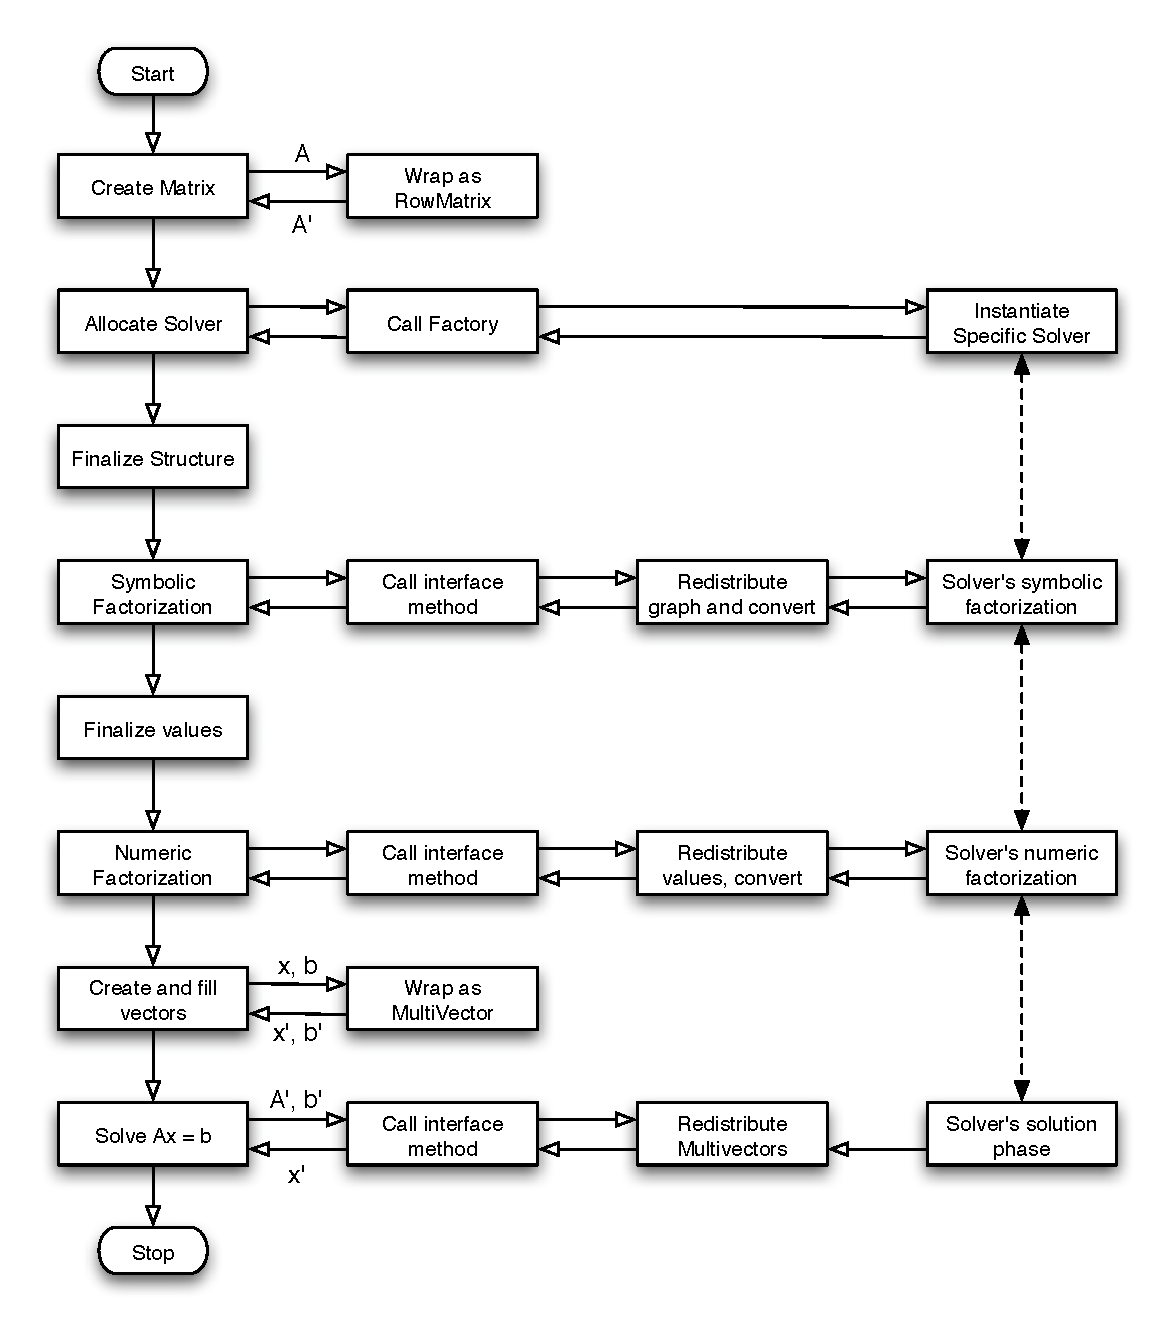
\includegraphics[width=12cm]{amesos_flowchart.eps}}
\end{center}
\caption{Flowchart of linear system solution. $A, x$ and $b$ represent objects
  defined in the application, while $A', x'$ and $b'$ are the corresponding 
    wrappers that
    satisfy Interfaces~\ref{int:vector} and \ref{int:ami}. Dashed lines mean
    that a given phase uses data defined in another phase. From left to right,
  the first colum 
    represents phases occurring in the application; the second column wrapping
and calls to generic interface methods; the third column actions
occurring in the solver interface, while the fourth column calls to supported
direct solver library.}
\label{fig:flowchart}
\end{figure}

Another observation not shown in Table~\ref{tab:packages} is that the matrix
format generally differs. Not all solvers can take advantage of
parallel environments; those that do 
(SuperLU\_DIST, DSCPACK, MUMPS, SPOOLES, WSMP) require different data layout
for matrix and
vectors. Moreover, the calling sequences are very different from one library
to the next.

Despite these differences, all solvers are accessed with a similar sequence of
steps:
\begin{enumerate}
\item Definition of the sparsity pattern of the linear system matrix;
\item Computation of the symbolic factorization;
\item Definition of the values of the linear system matrix;
\item Computation of the numeric factorization;
\item Definition of the values of the right-hand side;
\item Solution of the linear system.
\end{enumerate}
A flowchart of processes (1)-(6) is reported in Figure~\ref{fig:flowchart}.
While steps (1), (3) and (5) are application-dependent, steps (2), (4) and
(6) can be abstracted to define three phases: a {\sl symbolic
factorization}, a {\sl numeric factorization}, and a {\sl solve} phase. The
symbolic factorization refers to all operations that can be performed by
accessing the matrix structure only (without touching the matrix values);
numeric factorization refers to the construction of the factored terms, and
finally the solve phase is related to the computation of the solution vector
$X$ for a given $B$.

Our aim is to standardize steps (2), (4)
and (6) to allow a transparent and consistent usage
of most of the libraries of Table~\ref{tab:packages}, and makes it easy
to extend the support to other (new) projects. We are interested in the
following capabilities:
\begin{itemize}

\item {\sl Simplicity of usage:} Solving linear system (\ref{eq:linear_system}) in a language
like MATLAB is very easy, just write \verb!X = A \ B!. It should not be much
more difficult in a production code.

\item {\sl Flexibility:} More than one algorithm must be available,
  to offer optimal algorithms for small and large matrices, serial and
  parallel.

\item {\sl Efficiency:} The solution of (\ref{eq:linear_system}) must be as
efficient as possible, using state-of-the-art algorithms. Besides, the
overhead due to the design must be minimal.
\end{itemize}

To satisfy these goals, we introduces a set of abstract classes.

The first class that we need to introduce is a {\tt Map}, defined by
Interface~\ref{int:map}.
\begin{interface}
\label{int:map}
The {\tt Map} class will contain the following methods:

\begin{itemize}
\item {\tt int GetNumMyElements()} returns the number of locally owned elements;
\item {\tt int GetNumGlobalElements()} returns the global number of elements;
\item {\tt int GetGID(int LID)} returns the global ID of local node {\tt ID}.
\end{itemize}
\end{interface}
A {\tt Map} defines the local-to-global numbering. We require that any global
ID is assigned to exactly one processor. {\tt Map}'s are used to define the
layout of distributed vectors and matrices. Class {\tt Vector} defines a
distributed vector, which locally exists as a {\tt double} array.
A simple set of methods for the {\tt Vector} class is reported by Interface~\ref{int:vector}.

\begin{interface}
\label{int:vector}
The {\tt Vector} class will contain the following methods:

\begin{itemize}
\item {\tt double* GetValues()} returns a pointer to the local array of values;
\item {\tt Map\& GetMap()} returns a reference to the underlying Map object.
\end{itemize}
\end{interface}

For the sake of simplicity, this paper focuses on vectors and not on
multi-vectors (that is, a collection of vectors with the same {\tt Map}).
However, the presented design can be extended straightforwardly to tackle
multi-vectors.

\smallskip

The other distributed objects are matrices, here defined by the {\tt
  RowMatrix} class.  This class does not define a matrix format; instead, it
  specifies how to {\sl query} for matrix elements. Although converting a
  matrix from one given format to another is not a difficult operation,
we believe that forcing
users to adopt a specific matrix format is a burden that can slow down or
prevent the usage of a software library.

The {\tt RowMatrix} class is a fairly general matrix interface. For
distributed matrices, the only assumption is that each row is owned by exactly
one processor; rows can be distributed in arbitrary ways among the available
processors. This means that the locally owned matrix can be decomposed as
\begin{equation}
A^{(loc)}_i + A^{(ext)}_i,
\end{equation}
where $A^{(loc)}_i$ represents the square submatrix of elements whose row
and column correspond to locally hosted rows, while
$A^{(ext)}_i$ contains matrix elements with non-locally owned columns. The
columns contained in $A^{(ext)}$ are usually called {\sl ghost nodes}.
The abstract matrix interface is as
follows.
\begin{interface}
\label{int:ami}
The abstract interface to the distributed square matrix $A$
will contain the following methods:
\begin{itemize}
\item \verb!int GetNumMyRows()! returns the number of locally hosted rows;
\item \verb!int GetNumGlobalRows()! returns the global number of rows;
\item \verb!int GetNumGhostNodes()! returns the number of ghost nodes;
\item \verb!void GetUpdateGhostNodes(Vector& X)! updates the values of ghost nodes
 in the input vector {\tt X};
\item {\tt void GetMyRow(int ID, int\& NumEntries, int* Indices, double*
                             Values)} copies the
columns and values of all nonzero elements in locally hosted row 
in the user's allocated arrays.
\item \verb!Map& GetRowMap()! returns a reference to the map;
\item \verb!Map& GetColMap()! returns a reference to the map for the columns
(which contains the ghost elements).
\end{itemize}
\end{interface}

\smallskip

The last utility class we need to introduce is the {\tt Redistribute} class.
We suppose that, given two maps, called {\tt SourceMap} and {\tt TargetMap}, a
{\tt Redistribute} object can be used to redistribute a {\tt Vector} based on
{\tt SourceMap} to a vector based on {\tt TargetMap}. This class encapsulates
all the complexity of data communication.

\smallskip

The can now introduce the {\tt solver} interface class, which is defined as
follows:
\begin{interface}
\label{int:asi}
The {\tt Solver} interface
will contain the following methods:
\begin{itemize}
\item \verb!SetMatrix(RowMatrix* A)! sets the linear system matrix;
\item \verb!SetX(Vector* X)! sets the solution vector;
\item \verb!SetB(Vector* B)! sets the right-hand side vector;
\item \verb!SetParameters(List)! specifies all the parameters for the solver;
\item \verb!SymbolicFactorization()! performs the symbolic factorization, that
is, all the operations that do only require the matrix graph and not the
actual matrix values;
\item \verb!NumericFactorization()! performs the numeric factorization, that
is, computes the matrices $L$, $D$ and $U$ by accessing the matrix values.
Both the solution and the right-hand side are not required in this phase;
\item \verb!Solve()! solves the linear system. This phase requires the
solution and right-hand side vectors.
\end{itemize}
\end{interface}

%------------------------------------------------------------------------- 
\section{A Concrete Implementation}
\label{sec:concrete}
%------------------------------------------------------------------------- 

We now describe a concrete implementation of the proposed interfaces, as
available in the {\sl Amesos} package~\cite{Amesos-Reference-Guide}. 
Amesos,
developed by (in alphabetical order) T. Davis, M. Heroux, R. Hoekstra, M.
Sala, and K. Stanley, implements the abstract interfaces described in this
article. Amesos is distributed within the
Trilinos project~\cite{heroux05trilinos,trilinos-home-page}. Amesos is
configured using autoconf and autotools; each solver can be enabled at
configure time.

We have considered the following solvers among those
reported in Table~\ref{tab:packages}: KLU, UMFPACK, SuperLU, SuperLU\_DIST,
  DSCPACK, MUMPS, TAUCS, and PARDISO.
The considered libraries use different algorithms that are
representative of a far wider range of codes. Also, these supported libraries are
among the best codes publicly available, and are widely used.  In addition, we
have implemented an interface to the dense, serial solver LAPACK and an
interface to the dense, distributed solver ScaLAPACK.

\begin{figure}
\begin{center}
\begin{tabular}{| p{12cm} | }
\hline
 \\
\begin{minipage}{12cm}
\begin{verbatim}
#include "Amesos.h"
#ifdef HAVE_MPI
#include "mpi.h"
#include "Epetra_MpiComm.h"
#else
#include "Epetra_SerialComm.h"
#endif
...

int main(int argc, char *argv[]) 
{
#ifdef HAVE_MPI
  MPI_Init(&argc, &argv);
  Epetra_MpiComm Comm(MPI_COMM_WORLD);
#else
  Epetra_SerialComm Comm;
#endif

  Epetra_CrsMatrix* Matrix = <create matrix here>;
  Epetra_MultiVector* LHS = <create solution vector here>;
  Epetra_MultiVector* RHS = <create right-hand side here>; 

  Epetra_LinearProblem Problem(Matrix, LHS, RHS);

  Amesos Factory;                  // factory class
  string SolverType = "Umfpack";   // selected interface
  Amesos_BaseSolver* Solver;       // generic solver object
  Solver = Factory.Create(SolverType, Problem);

  Teuchos::ParameterList List;     // allocate container for params,
  List.set("PrintTiming", true);   // set one in the container, then
  Solver->SetParameters(List);     // pass the container to the solver

  Solver->SymbolicFactorization(); // symbolic factorization
  Solver->NumericFactorization();  // numeric factorization
  Solver->Solve();                 // linear system solution

  delete Solver;
    
#ifdef HAVE_MPI
  MPI_Finalize();
#endif
  return(EXIT_SUCCESS);
} // end of main()
\end{verbatim}
\end{minipage} \\
 \\
 \hline
\end{tabular}
\caption{Example of code using Amesos. The code uses the Amesos interface to
  UMFPACK to solve the linear system. The creation of the matrix, solution and
    right-hand side are not reported. {\tt HAVE\_MPI} is a compilation macro
    that specifies the usage or not of the MPI library.}
\label{fig:example}
\end{center}
\end{figure}

\begin{figure}
\begin{center}
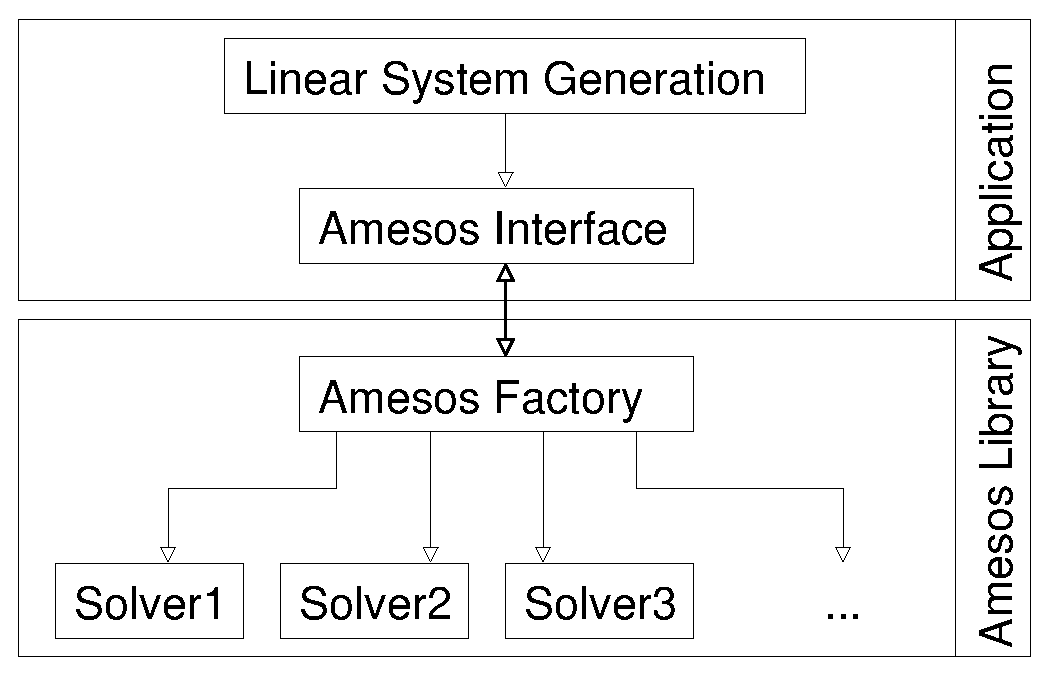
\includegraphics[width=7cm]{amesos_and_application.eps}
\end{center}
\caption{Connection between a generic application and Amesos.}
\label{fig:app}
\end{figure}

An example of usage of Amesos is reported in Figure~\ref{fig:example}. The
code can be compiled with or without support for MPI. (Clearly, distributed
solvers are available only when Amesos is compiled with MPI support.) The only
Amesos include is \verb!Amesos.h!, which does not include the header files of
the supported library. The selected interface is specified by the string
variable \verb!SolverType!, and the required interface is created by using the
factory class \verb!Amesos!. Factory classes are a programming
tool (see~\cite{alexandrescu01modern}) that implement a sort of ``virtual
constructor,'' in the sense that one can instantiate a derived (concrete) object
while still working with abstract types.
 
Once the required interface is created, the symbolic factorization is
performed by calling \verb!Solver->SymbolicFactorization()!.
This phase does not require the numerical values of \verb!A!, which can
therefore be changed after the call to \verb!SymbolicFactorization()!.
However,  the nonzero pattern of \verb!A! {\em cannot} be
changed.
The numeric factorization is performed by
\verb!Solver->NumericFactorization()!, which
accesses the values of \verb!A!, but does not
consider the vectors \verb!X! and \verb!B!. Finally, the instruction
\verb!Solver->Solve()! solves the linear system and stores in \verb!LHS! the
solution of the linear system.

Each Amesos interface automatically selects the default parameters defined by
the supported solver. In most cases, these values are a robust and reliable
choice for most applications. If required, the user can tune some of the
parameters by using method \verb!SetParameters()!.

Example of Figure~\ref{fig:example} adopts UMFPACK as a solver; other
interfaces can be created using the factory class by simply changing one
parameter. Note that the supported solver can be serial or parallel, dense or
sparse: the user code still remains the same (except for the name of the
                                              solver); Amesos will take care
of data redistribution if required by the selected solver. Therefore, a
generic interface between an application code and Amesos is as represented in
Figure~\ref{fig:app}: Once $A$, $X$ and $B$ of (\ref{eq:linear_system}) are
available, then the application can use the factory class to access the
supported libraries.

% ------------------------------------------------------------------------
\section{Numerical Results}
\label{sec:numerical}
% ------------------------------------------------------------------------

C++ codes are usually considered elegant but inefficient; therefore, this
section reports some numerical results to quantify the additional CPU time
required by the general classes presented in Section~\ref{sec:design} and
implemented by the Amesos project of Section~\ref{sec:concrete}.

Figure~\ref{fig:results} reports the percentage of CPU time required by the Amesos
interface with respect to the time required by the library itself, 
  for matrices obtained from the FIDAP collection, available
at~\cite{matrix-market}. The considered sizes go from 27 
({\tt FIDAP005}) to 22294 ({\tt FIDAPM11}). All problems are solved using one
1.67 GHz G4 processor with 1024 Mbytes of RAM, running MAC OS X 10.4 and gcc
4.0.0. We have considered the (serial) solvers UMFPACK and
SuperLU. The table reports the percentage of the CPU time required by the
interface with respect to the time required by the considered solver, and
quantifies the overhead required by Amesos. We have used to default set of
parameters for all solvers.

For the smallest matrices (like \verb!FIDAP005! or \verb!FIDAPM05!, of size
27 and 42, respectively)
the overhead is considerable, while for most of the others the amount of
overhead is below 5\%. The interface still require significant overhead of
relatively big matrices, and this is probably because these matrices are quite
easy to solve (and therefore the CPU time spent in the solver is small).
For the biggest matrices the overhead is often below 1\%.

\begin{figure}
\begin{center}
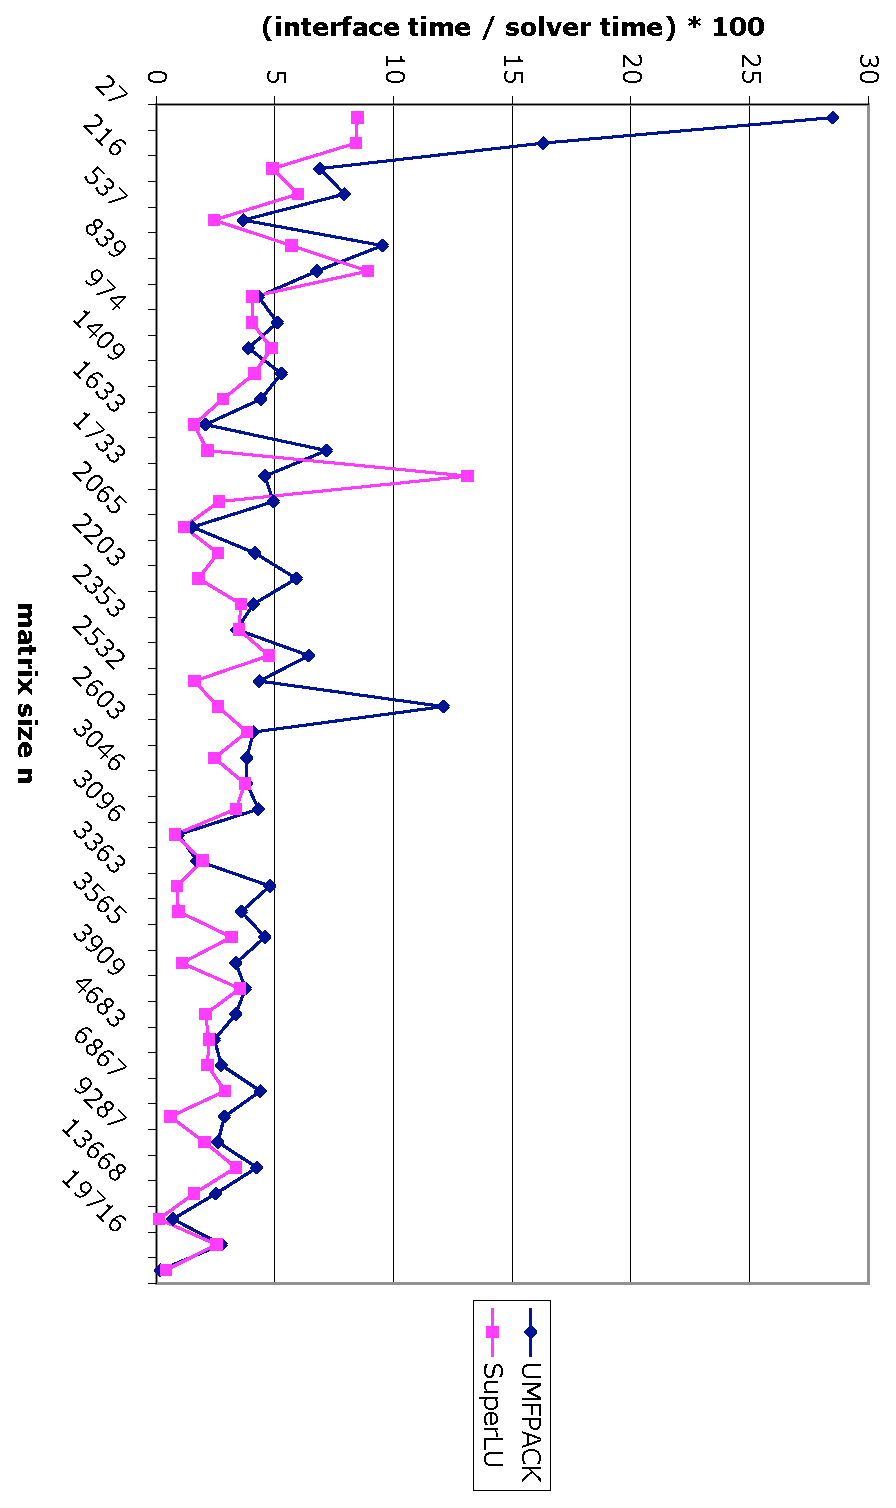
\includegraphics[angle=90,width=13cm]{interface_time.eps}
\caption{Additional time required by the Amesos interface with respect to the
time required by the solver, for different matrices and solvers. $n$
  represents the size of the matrix, and $nnz$ the total number of nonzeros.
The results were obtained on a G4 1.67 GHz with 1 GByte of RAM.}
\label{fig:results}
\end{center}
\end{figure}

%-----------------------------------------------------------------------------
\section{Examples of Applications}
\label{sec:example}
%-----------------------------------------------------------------------------

%-----------------------------------------------------------------------------
\subsection{Applications to Domain Decomposition and Multilevel Preconditioners}
\label{sec:preconditioner}
%-----------------------------------------------------------------------------

For an abstract point of view, an algebraic domain decomposition
preconditioner for the iterative solution of the linear system
(\ref{eq:linear_system})
if any preconditioner $B$ that can be written as
\begin{equation}
\label{eq:prec}
B^{-1} = \sum_{i=1}^M P'_i {A'_i}^{-1} R_i.
\end{equation}
Let $V = \mathbb{R}^n$, and
let $V_i \subset V, i = 1, \ldots, M$ be a decomposition of $V$, such that
$\cup_{i=1}^M V_i = V$, and $R_i: V \rightarrow V_i$ a restriction operator
from $V$ to the subspace $i$ (of size $n_i$),
and $P_i: V_i \rightarrow V, P'_i : V_i \rightarrow V$ two prolongator
operators. $A'_i$ is an approximation to $A_i = R_i A P_i$.  We refer to 
monographs~\cite{QV2,smith96parallel} for a detailed
overview of domain decomposition methods, to~\cite{saad96iterative} for the
algebraic interpretation.

One disadvantage of one-level domain decomposition preconditioners is that
their performances deteriorate as the number of subdomains increases.
Therefore, these preconditioners are completed by one or more additional
(coarser) levels, as done in two-level domain decomposition preconditioners or
in multilevel methods; 
see for instance \cite{brandt.classic,hack.book,hack2.book}. 

Direct solution methods can be required in two phases: In the application of
the $A'_i$'s, and in the solution of the coarse problem. In both cases, it
suffices to wrap the $A'_i$'s or the coarse matrix to satisfy
Interface~\ref{int:ami} to access any of the library supported by Amesos using
a sequence of instructions that
basically look like the one of Figure~\ref{fig:example}, with the only
difference
that the vectors \verb!LHS! and \verb!RHS! must be specified just before a
call to \verb!Solve()!.  The libraries
IFPACK~\cite{ifpack-guide} and ML~\cite{ml-guide} are two examples of
preconditioning packages adopt this approach.

%-----------------------------------------------------------------------------
\subsection{Scripting Language Interface: PyAmesos}
\label{sec:pyamesos}
%-----------------------------------------------------------------------------

Another advantage of the presented set of interface is that is it (relatively)
  easy to use them from a scripting language like Python by adopting tools
  like SWIG~\cite{swig}. Since SWIG supports intra-language class inheritance,
  it is possible to derive Interface~\ref{int:ami} in Python, then pass it
  to the Python wrapper of Interface~\ref{int:asi}. This approach makes all the
  supported libraries available to Python developers at almost no cost. For
  more details, we refer to the PyTrilinos
  documents~\cite{sala05pytrilinos,pytrilinos-la-guide}. 
An example of usage is reported in Figure~\ref{fig:pyamesos}. The example
reads a matrix in Harwell/Boeing format, distributes it linearly across the
available processors, then calls MUMPS to solve the linear system. Python's
dictionaries are used to specify parameters (in this case, the level of
                                             output). After solution, the
script computes the 2-norm of the error.

\begin{figure}
\begin{center}
\begin{tabular}{| p{12cm} |}
\hline
\\
\footnotesize
\begin{minipage}{11.5cm}
\begin{verbatim}
#! /usr/bin/env python
try:
  from PyTrilinos import Amesos, Triutils, Epetra
except ImportError:
  raise ImportError, "error w/ Amesos or Triutils or Epetra"

Comm = Epetra.PyComm()
Map, Matrix, LHS, RHS, Exact = Triutils.ReadHB("fidap035.rua", Comm)

Problem = Epetra.LinearProblem(Matrix, LHS, RHS);
Factory = Amesos.Factory()
SolverType = "MUMPS"
Solver = Factory.Create(SolverType, Problem)
AmesosList = {
  "PrintTiming": True,
  "PrintStatus": True
}
Solver.SetParameters(AmesosList)
Solver.SymbolicFactorization()
Solver.NumericFactorization()
Solver.Solve()
LHS.Update(-1.0, Exact, 1.0)
norm = LHS.Norm2()
print '||x_computed - x_exact||_2 = ', norm[1]
\end{verbatim}
\end{minipage}
\\
\\
\hline
\end{tabular}
\caption{Complete script that solves a linear system using Amesos/MUMPS in
  Python.}
\label{fig:pyamesos}
\end{center}
\end{figure}

%-----------------------------------------------------------------------------
\section{Concluding Remarks}
\label{sec:conclusions}
%-----------------------------------------------------------------------------

In this paper, we have presented a model to access direct
solver libraries. The model is composed by two abstract interfaces, one to
access the matrix elements, and the other to manage each library.
The advantages of this model are:
\begin{itemize}

\item The actual data storage of linear system matrix becomes inessential.
Each concrete implementation will take care, if necessary, to convert the
input matrix into the required data format, should the row access provided by
\verb!GetMyRow()! method be not sufficient. This means that the
application can choose the matrix format independently as long as the abstract
matrix interface is implemented.

\item Issues like diagonal perturbations, reordering or dropping before the
factorization can be easily introduced within the abstract matrix interface.
For example, a dropping strategy or a modification of the diagonals simply
requires a new \verb!GetMyRow()! method, without touching the actual matrix
storage.

\item The actual calling sequence required by each library to factorize the
matrix and solve the linear system becomes inessential. Instead, the user only
has to call methods \verb!SymbolicFactorization()!, \verb!NumericFactorization()! and
\verb!Solve()!.

\item Interfaces can be tested more easily because they are all located within
the same library and not spread out into several application codes.
\end{itemize}

Clearly,  generalities comes at a price: The presented model has the following
limitations:
\begin{itemize}
\item 
Each interface automatically selects the default parameters defined by the
supported solver. In most cases, these values are a robust and reliable choice
for most applications. If required, the user can tune some of the parameters
by using method \verb!SetParameters()!. However, some fine-tuning can be
difficult since Interface~\ref{int:asi} has no knowledge of the underlying
solver data structure.

\item There
  is no standard way to 
  convert MPI communicators defined in C to MPI communicators defined
  in FORTRAN90. On some architectures it is difficult or even
  impossible to perform such a task. Some hacks may be required.

\item 
It is almost impossible to support different versions of a given software
library, because
function names usually do not vary from one version to the
next, making it impossible for the linker to select the
  appropriate version of the library.

\item 
Not all interfaces can be compiled and linked at the same time. Often
developers of direct solver libraries take advantage of other, smaller
libraries, that offer common functionalities. Typically, this happens with
reordering algorithms. Unfortunately,
it is not uncommon for different solver libraries to request different
versions of a given reordering algorithm, all codes using the same function
names. As a result, not all the interfaces can be compiled and used at the
same time.
\end{itemize}

%The reader might wonder why we have limited our attention to direct methods only, and
%we did not include iterative methods as well in the definition of the abstract
%interfaces. The reason is that, although
%being often more performant in terms of CPU time and memory usage, iterative
%solvers are less robust and mich less black-box than direct methods. Most
%iterative methods are developed for PDE-like problems, and might have poor
%performances if applied to more general matrices. However, libraries based on
%the abstract matrix interface exist.
%
%\smallskip

Despite these problems, we believe that the presented set of interfaces
bring their users the well-known benefits of reusable libraries. Thanks to
their generality, these interfaces (and the corresponding code) can be used to
easily connect intricate applications with state-of-the-art linear solver
libraries, in a simple and easy-to-maintain way. From the point of view of
application developers, the small amount of required code makes it very
convenient to adopt a project like Amesos. For linear solver
libraries' developers  writing one interface for their own solver can help to make it
applicable and testable to a vast range of applications.

In our opinion, the only limitation of Amesos is that it supports double
precision only, while most direct solvers allows the solution in single
precision and complex arithmetics.  Although the model can in principle
support single precision and complex arithmetics (by using templates, for
                                                  example), no code that
implements Interface~\ref{int:asi} has been written yet. A templated version
of Interface~\ref{int:ami} is under development.

%-----------------------------------------------------------------------------%
\section*{Acknowledgments}
%-----------------------------------------------------------------------------%

The authors wish to thank M.~Heroux, R.~Hoekstra and T.~Davis for several
fruitful discussions and suggestions about the organization of the Amesos
project. Part of the work has been conducted under the financial support of
the Sandia National Laboratories.

%-----------------------------------------------------------------------------%
\bibliographystyle{acmtrans}
\bibliography{paper}
%-----------------------------------------------------------------------------%

\end{document}

\begin{table}
\begin{center}
\begin{tabular}{|l r r r| r r r|}
\hline
\multicolumn{4}{| c |}{Matrix} &
\multicolumn{3}{ c |}{Interface Time / Solver Time * 100} \\
Name  & $n$   & $nnz$  & $nnz / n$  & KLU     & UMFPACK   & SuperLU \\
\hline
\tt FIDAP001 & 216   &   4374 & 20.25 & 23.5   & 6.89  & 4.89  \\
\tt FIDAP002 & 414   & 26831  & 60.84 & 26.6   & 7.92  & 5.96  \\
\tt FIDAP003 & 1821  & 52659  & 28.91 & 18.5   & 4.94  & 2.64  \\
\tt FIDAP004 & 1601  & 32287  & 20.16 & 1.47   & 4.40  & 2.81  \\
\tt FIDAP005 & 27    & 279    & 10.33 & 112.52 & 28.5  & 8.46  \\
\tt FIDAP006 & 1651  & 49479  & 29.96 & 1.03   & 7.17  & 2.14  \\
\tt FIDAP007 & 1633  & 54487  & 33.36 & 12.8   & 2.07  & 1.59  \\
\tt FIDAP008 & 3096  & 106302 & 34.33 & 10.8   & 0.931 & 0.789 \\
\tt FIDAP009 & 3363  & 99397  & 29.55 & 14.6   & 4.78  & 0.863  \\  
\tt FIDAP010 & 2410  & 54816  & 22.74 & 25.78  & 6.43  & 4.75  \\  
\tt FIDAP011 & 16614 &1091362 & 65.68 & 0.120  & 0.701 & 0.111 \\  
\tt FIDAP012 & 3973  & 80151  & 20.17 & 0.216  & 3.34  & 2.07  \\  
\tt FIDAP013 & 2568  & 75628  & 29.45 & 18.31  & 12.1  & 2.59  \\  
\tt FIDAP014 & 3251  & 66647  & 20.50 & 0.172  & 1.71  & 1.94  \\  
\tt FIDAP015 & 6867  & 96421  & 14.04 & 10.480 & 4.38  & 2.89  \\  
\tt FIDAP018 & 5773  & 69335  & 12.01 & 8.18   & 2.73  & 2.14  \\  
\tt FIDAP019 & 12005 & 259863 & 21.64 & 15.17  & 4.23  & 3.34  \\  
\tt FIDAP020 & 2203  & 69579  & 31.58 & 1.32   & 5.89  & 1.77  \\  
\tt FIDAP021 & 656   & 19142  & 29.17 & 6.84   & 9.52  & 5.68  \\  
\tt FIDAP022 & 839   & 22613  & 26.95 & 6.50   & 6.76  & 8.92  \\
\tt FIDAP023 & 1409  & 43481  & 30.85 & 0.934  & 5.26  & 4.13  \\
\tt FIDAP024 & 2283  & 48733  & 21.34 & 2.11   & 4.09  & 3.55  \\
\tt FIDAP025 & 848   & 24532  & 28.92 & 9.93   & 4.29  & 4.04  \\
\tt FIDAP026 & 2163  & 93749  & 43.34 & 0.724  & 4.16  & 2.59  \\
\tt FIDAP027 & 974   & 40736  & 41.82 & 5.25   & 5.10  & 4.02  \\
\tt FIDAP028 & 2603  & 77653  & 29.83 & 0.896  & 4.08  & 3.81  \\
\tt FIDAP029 & 2870  & 23754  & 8.276 & 9.95   & 3.81  & 2.44  \\
\tt FIDAP031 & 3909  & 115299 & 29.49 & 0.575  & 3.75  & 3.51  \\
\tt FIDAP032 & 1159  & 11343  & 9.786 & 0.791  & 3.87  & 4.84  \\
\tt FIDAP033 & 1733  & 20315  & 11.72 & 15.89  & 4.58  & 13.1   \\
\tt FIDAP035 & 19716 & 218308 & 11.07 & 8.56   & 2.74  & 2.53  \\
\tt FIDAP036 & 3079  & 53851  & 17.48 & 2.03   & 4.30  & 3.35  \\
\tt FIDAP037 & 3565  & 67591  & 18.95 & 11.08  & 4.58  & 3.15  \\
\tt FIDAPM02 & 537   & 19241  & 35.83 & 14.74  & 3.67  & 2.42  \\
\tt FIDAPM03 & 2532  & 50380  & 19.89 & 1.00   & 4.33  & 1.61  \\
\tt FIDAPM05 & 42    & 520    & 12.38 & 82.85  & 16.3  & 8.40  \\
\tt FIDAPM07 & 2065  & 53533  & 25.92 & 0.602  & 1.52  & 1.15  \\
\tt FIDAPM08 & 3876  & 103076 & 26.59 & 0.220  & 3.36  & 1.08  \\
\tt FIDAPM09 & 4683  & 95053  & 20.29 & 0.536  & 2.45  & 2.21  \\
\tt FIDAPM10 & 3046  & 53842  & 17.67 & 9.979  & 3.82  & 3.72  \\
\tt FIDAPM11 & 22294 & 623554 & 27.96 & N/C    & 0.17  & 0.403 \\
\tt FIDAPM03 & 3549  & 71975  & 20.28 & 0.355  & 3.59  & 0.919 \\
\tt FIDAPM05 & 9287  & 98519  & 10.60 & 42.90  & 2.59  & 2.03  \\
\tt FIDAPM29 & 13668 & 186294 & 13.62 & 0.869  & 2.511 & 1.57  \\
\tt FIDAPM33 & 2353  & 23765  & 10.09 & 0.6560 & 3.39  & 3.47  \\
\tt FIDAPM37 & 9152  & 765944 & 83.69 & 2.247  & 2.87  & 0.585 \\
\hline
\end{tabular}
\end{center}
\end{table}

